% !TEX root = main.tex
\section{Obecny stan i dalszy rozwój narzędzia GenericMonitoringTool}
Narzędzie GenericMonitoringTool jest szeroko i chętnie wykorzystywane w ramach platformy Athena, na potrzeby tworzenia histogramów i monitorowania kodu.
W momencie pisania tej pracy, w jej kodzie zadeklarowanych jest ponad 450 zmiennych monitorowanych w obrębie 53 różnych algorytmów. 
Mogą one wypełnić danymi prawie 4500 zdefiniowanych histogramów.
Do tej pory nie zostały zgłoszone żadne krytyczne błędy, które uniemożliwiałyby pracę z tym narzędziem.

Obecnie toczą się prace nad dodawaniem nowych funkcjonalności do kodu GenericMonitoringTool.
Mają one na celu pokrycie dodatkowych przypadków użycia, dzięki którym możliwe będzie dotarcie do większej liczby użytkowników. 
Został on również szeroko wykorzystany podczas technicznego "reprocessingu" dla 22 wersji platformy Athena, dla którego przykładowe histogramy zostały przedstawione na \figref{fig:athena:histogram_TH1}, \figref{fig:athena:histogram_TH1_time} i \figref{fig:athena:histogram_TH2}.

\begin{figure}[!ht]
\centering
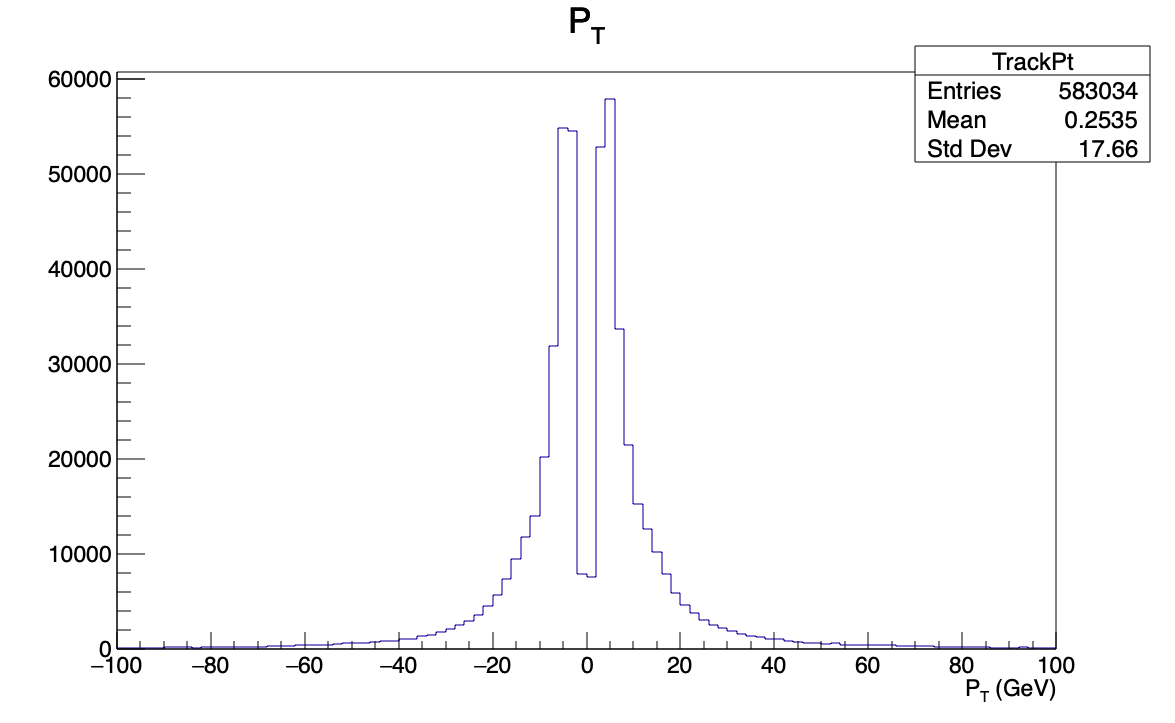
\includegraphics[width=1\textwidth]{img/histogram_TH1.png}
\caption{
Przykładowy histogram TH1 dla zmiennej monitorowanej typu 'Scalar', utworzony z pomocą GenericMonitoringTool. /// PT ped poprzeczny * ładunek
}
\label{fig:athena:histogram_TH1}
\end{figure}

\begin{figure}[!ht]
\centering
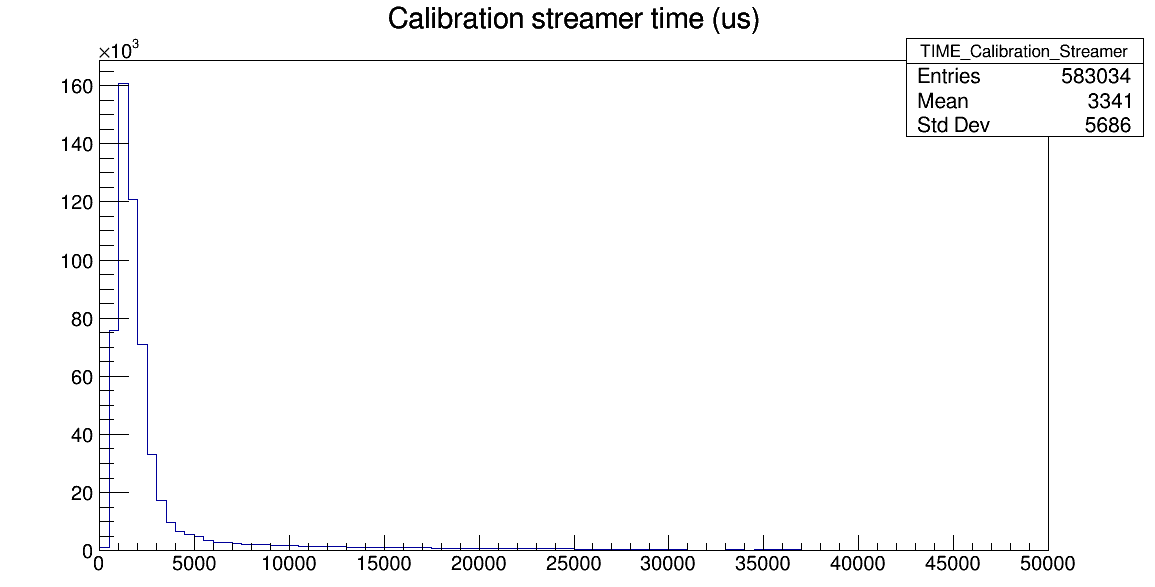
\includegraphics[width=1\textwidth]{img/histogram_TH1_time.png}
\caption{
Przykładowy histogram TH1 dla zmiennej monitowanej typu 'Timer', utworzony z pomocą GenericMonitoringTool 
}
\label{fig:athena:histogram_TH1_time}
\end{figure}

\begin{figure}[!ht]
\centering
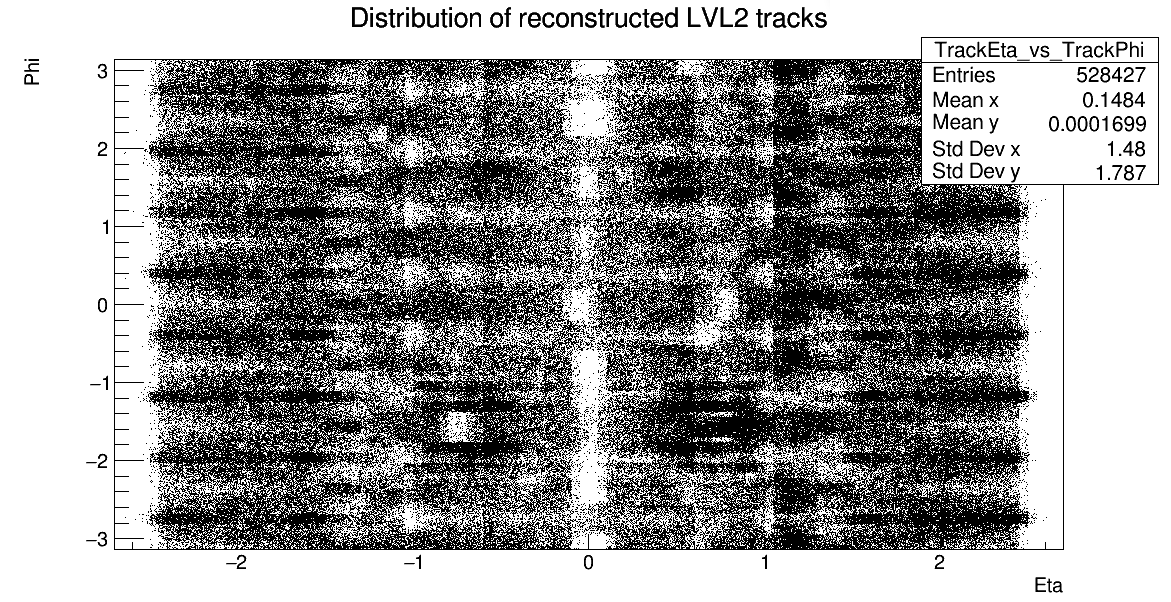
\includegraphics[width=1\textwidth]{img/histogram_TH2.png}
\caption{
Przykładowy histogram TH2 dla dwóch zmiennych monitowanych typu 'Scalar', utworzony z pomocą GenericMonitoringTool /// colz box opcje histogramu root /// mapa zrekonsturowanych sladow
}
\label{fig:athena:histogram_TH2}
\end{figure}

\begin{python}[caption=Deklaracja histogramów, label={lst:athena:histogram_declaration}]
class TrigL2MuonSAMonitoring(GenericMonitoringTool):
    def __init__ (self, name = "TrigL2MuonSAMonitoring"):
        super(TrigL2MuonSAMonitoring, self).__init__( name )
    
        self.HistPath = name
(*@\centerline{\raisebox{-1pt}[0pt][0pt]{$\vdots$}}@*)
        self.defineHistogram('TrackPt', type='TH1F', path='EXPERT', title="P_{T};P_{T} (GeV)", xbins=100, xmin=-100, xmax=100 )
(*@\centerline{\raisebox{-1pt}[0pt][0pt]{$\vdots$}}@*)
        self.defineHistogram('TrackEta, TrackPhi', type='TH2F', path='EXPERT', title="Distribution of reconstructed LVL2 tracks; Eta; Phi", xbins=108, xmin=-2.7, xmax=2.7, ybins=96, ymin=-3.1416, ymax=3.1416 )
(*@\centerline{\raisebox{-1pt}[0pt][0pt]{$\vdots$}}@*)
        self.defineHistogram('TIME_Calibration_Streamer', type='TH1F', path='EXPERT', title="Calibration streamer time (us)", xbins=100, xmin=0, xmax=50000 )
\end{python}

\begin{cpp}[caption=TIME Calibration Streamer, label={lst:athena:time_calibration_streamer}]
StatusCode MuFastSteering::findMuonSignature(
  const DataVector<const TrigRoiDescriptor>& roids,
  const DataVector<const LVL1::RecMuonRoI>& muonRoIs,
  DataVector<xAOD::L2StandAloneMuon>& outputTracks,
  TrigRoiDescriptorCollection& outputID,
  TrigRoiDescriptorCollection& outputMS,
  DataVector<xAOD::TrigComposite>& outputComposite )
{
(*@\centerline{\raisebox{-1pt}[0pt][0pt]{$\vdots$}}@*)
  auto calibrationTimer = Monitored::Timer( "TIME_Calibration_Streamer" );

  auto monitorIt	= Monitored::Group(m_monTool, prepTimer, patternTimer, stationFitterTimer, trackFitterTimer, trackExtraTimer, calibrationTimer );
(*@\centerline{\raisebox{-1pt}[0pt][0pt]{$\vdots$}}@*)
  calibrationTimer.start();
(*@\centerline{\raisebox{-1pt}[0pt][0pt]{$\vdots$}}@*)
  sc = m_calStreamer->createRoiFragment(*p_roi,tp,m_mdtHits_normal, m_rpcHits, m_tgcHits, m_calBufferSize, m_calDataScouting, updateTriggerElement); 
(*@\centerline{\raisebox{-1pt}[0pt][0pt]{$\vdots$}}@*)
  calibrationTimer.stop();
(*@\centerline{\raisebox{-1pt}[0pt][0pt]{$\vdots$}}@*)
}
\end{cpp}

\begin{cpp}[caption=TrackPt, label={lst:athena:track_pt}]
StatusCode MuFastSteering::updateMonitor(const LVL1::RecMuonRoI* roi,
  const TrigL2MuonSA::MdtHits& mdtHits,
  std::vector<TrigL2MuonSA::TrackPattern>& trackPatterns )
{
(*@\centerline{\raisebox{-1pt}[0pt][0pt]{$\vdots$}}@*)
  auto track_pt 	= Monitored::Scalar("TrackPt", 9999.);
(*@\centerline{\raisebox{-1pt}[0pt][0pt]{$\vdots$}}@*)
  auto monitorIt	= Monitored::Group(m_monTool, inner_mdt_hits, middle_mdt_hits, outer_mdt_hits, invalid_rpc_roi_number, efficiency, sag_inverse, address, absolute_pt, sagitta, track_pt, track_eta, track_phi, failed_eta, failed_phi, res_inner, res_middle, res_outer, fit_residuals );
(*@\centerline{\raisebox{-1pt}[0pt][0pt]{$\vdots$}}@*)
  track_pt = (fabs(pattern.pt ) > ZERO_LIMIT) ? pattern.charge*pattern.pt : 9999.;
  absolute_pt = fabs(track_pt);
(*@\centerline{\raisebox{-1pt}[0pt][0pt]{$\vdots$}}@*)
}
\end{cpp}

\begin{cpp}[caption=TrackEta vs TrackPhi, label={lst:athena:track_eta_vs_track_phi}]
StatusCode MuFastSteering::updateMonitor(const LVL1::RecMuonRoI* roi,
  const TrigL2MuonSA::MdtHits& mdtHits,
  std::vector<TrigL2MuonSA::TrackPattern>& trackPatterns )
{
(*@\centerline{\raisebox{-1pt}[0pt][0pt]{$\vdots$}}@*)
  std::vector<float> t_eta, t_phi;
(*@\centerline{\raisebox{-1pt}[0pt][0pt]{$\vdots$}}@*)
  t_eta.clear();
  t_phi.clear();
(*@\centerline{\raisebox{-1pt}[0pt][0pt]{$\vdots$}}@*)
  auto track_eta	= Monitored::Collection("TrackEta", t_eta);
  auto track_phi	= Monitored::Collection("TrackPhi", t_phi);
(*@\centerline{\raisebox{-1pt}[0pt][0pt]{$\vdots$}}@*)
  auto monitorIt	= Monitored::Group(m_monTool, inner_mdt_hits, middle_mdt_hits, outer_mdt_hits, invalid_rpc_roi_number, efficiency, sag_inverse, address, absolute_pt, sagitta, track_pt, track_eta, track_phi, failed_eta, failed_phi, res_inner, res_middle, res_outer, fit_residuals );
(*@\centerline{\raisebox{-1pt}[0pt][0pt]{$\vdots$}}@*)
  if ( fabs(pattern.etaMap) > ZERO_LIMIT || fabs(pattern.phiMS) > ZERO_LIMIT ) {
    t_eta.push_back(pattern.etaMap);
    t_phi.push_back(pattern.phiMS);
  }
(*@\centerline{\raisebox{-1pt}[0pt][0pt]{$\vdots$}}@*)
}
\end{cpp}

W przyszłości, planowana jest m.in. aktualizacja framworka ROOT.
Jego najnowsze wersje zapewniają bezpieczeństwo dla przetwarzania wielowątkowego i wieloprocesowego. 
Taka zmiana pozwoli usunąć niepotrzebne sekcje krytyczne z kodu GenericMonitoringTool.

\subsection{Zastosowanie w systemie wyzwalania online}
//TODO
\subsection{Zastosowanie do monitorowania offline - Data Quality}
//TODO~\cite{atlas-multithread-article}
\subsection{Możliwe kierunki rozwoju}
//TODO
